\section{$\text{H}_2$/$\text{O}_2$ reaction kinetics: high-dimensional case}
\label{sec:app}

For the high-dimensional case, we aim to investigate the impact of the uncertain
pre-exponents ($A_i$'s) as well as the activation energies ($E_{a,i}$'s) on ignition 
delay during the H$_2$/O$_2$ reaction. The $A_i$'s are considered to be uniformly
distributed in the interval, $[0.9A_i^\ast, 1.1A_i^\ast]$. The $E_{a,i}$'s for all
reactions except $\mathcal{R}_6$ -- $\mathcal{R}_9$ and $\mathcal{R}_{13}$
are considered to be uncertain and uniformly distributed in the interval: 
$[0.99E_{a,i}^\ast, 1.01E_{a,i}^\ast]$. The nominal values, $A_i^\ast$ and $E_{a,i}^\ast$
corresponding to the different reaction rates are provided in~\cite{Yetter:1991}. 

The gradient-free approach discussed earlier in~\ref{sub:gradfree} was used to compute the
active subspace. Using the iterative procedure, the convergence of the eigenvectors
was examined by tracking $\delta \hat{\mat{W}}_{1,j}^{(i)}$. In Figure~\ref{fig:conv_app} (left),
components of the converged eigenvector based on 50 samples using $\tau$ = 0.2 are plotted.
To illustrate convergence, we compare them with components of the eigenvector obtained
using 100 samples (twice as many). The variation of maximum $\delta w_{1,j}^{(i)}$ between
successive iterations during the course of the iterative procedure is illustrated in 
Figure~\ref{fig:conv_app} (right). 
%
\begin{figure}[htbp]
 \begin{center}
  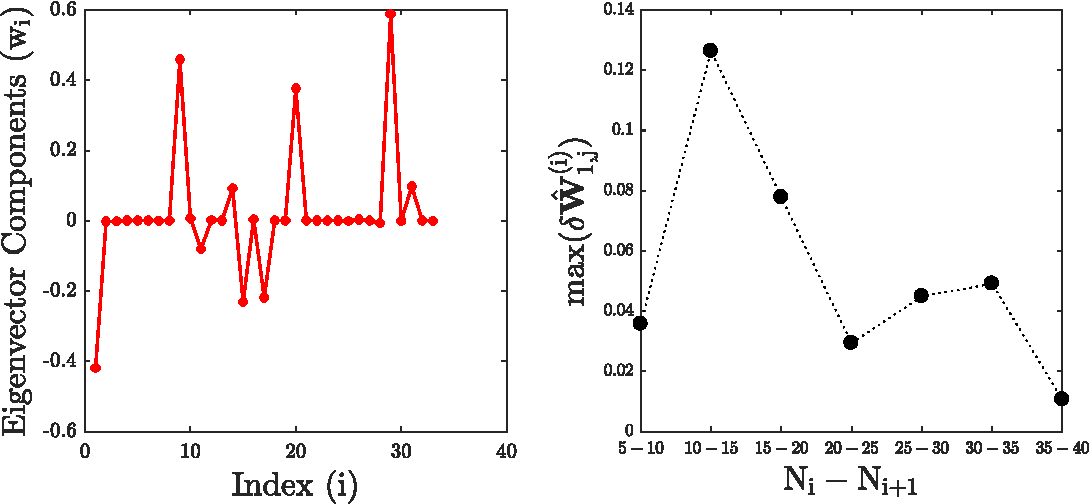
\includegraphics[width=0.8\textwidth]{./Figures/eigv10}
\caption{Left: An illustrative comparison of individual components of the converged dominant eigenvector obtained
using the two approaches discussed in~\ref{sub:grad} and~\ref{sub:gradfree}. Right: The quantity,  $\delta \hat{\mat{W}}_{1,j}^{(i)}$
is plotted for successive iterations to illustrate the convergence behavior.}
\label{fig:conv_app}
\end{center}
\end{figure}
%
The dominant eigenvector is observed to converge with only 50 samples in the 33-dimensional space which is remarkably efficient. 

In Figure~\ref{fig:hd}, we illustrate the resulting eigenvalue spectrum and the sufficient summary 
plot.
%
\begin{figure}[htbp]
 \begin{center}
   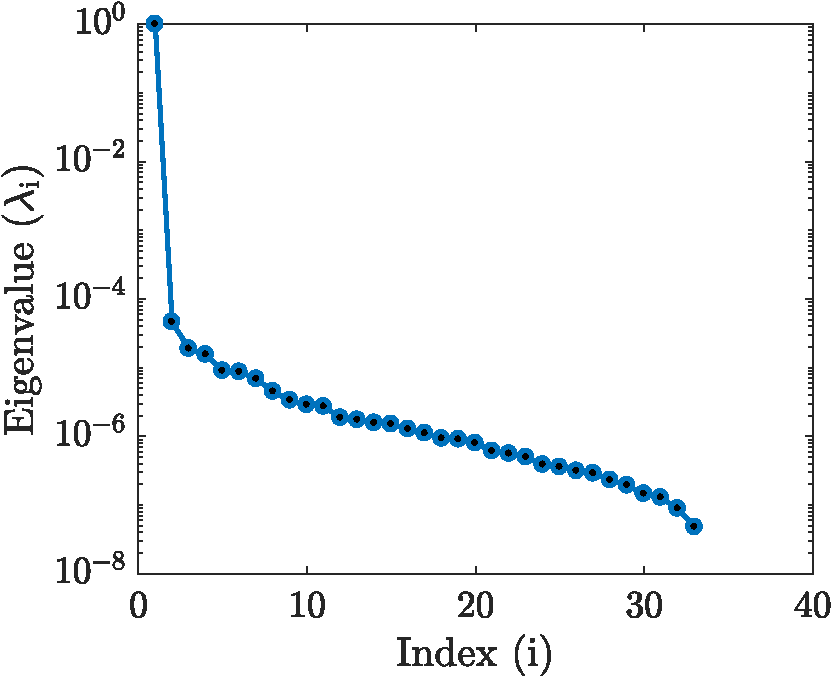
\includegraphics[width=0.45\textwidth]{./Figures/eig_33D}
   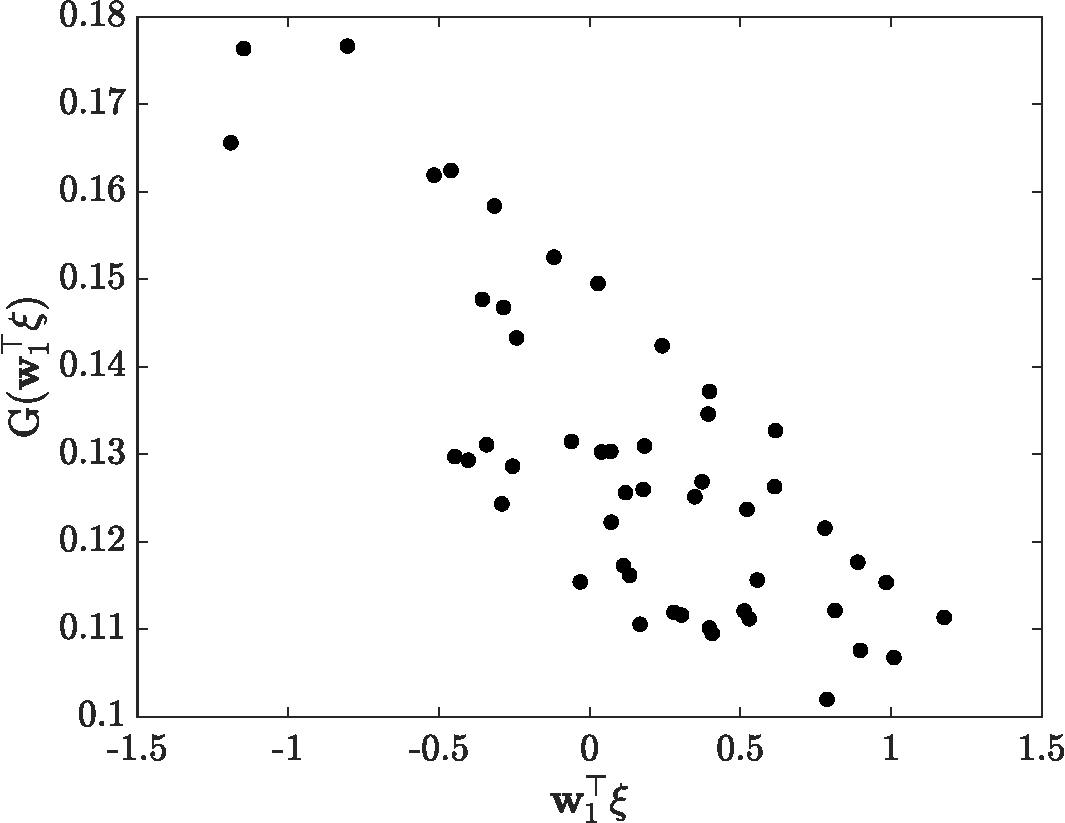
\includegraphics[width=0.45\textwidth]{./Figures/ssp_33D}
\caption{Left: Eigenvalue spectrum of $\hat{\mat{C}}$. Right: Sufficient summary plot indicating the
existence of a potential 1-dimensional active subspace.} 
\label{fig:hd}
\end{center}
\end{figure}
%
The second eigenvalue is observed to be roughly four orders of magnitude smaller than the first 
indicating the existence of a 1-dimensional active subspace. This is further confirmed by the sufficient
summary plot which shows that the variability in $G$ can be approximated using a 1-dimensional regression
fit which could be used as a surrogate. We will verify the accuracy of the surrogate later in~\ref{sub:verify}.

Components of the dominant eigenvector in Figure~\ref{fig:conv_app} (left) are used for estimating the
activity scores, plotted below in Figure~\ref{fig:as_33D}.
%
\begin{figure}[htbp]
 \begin{center}
  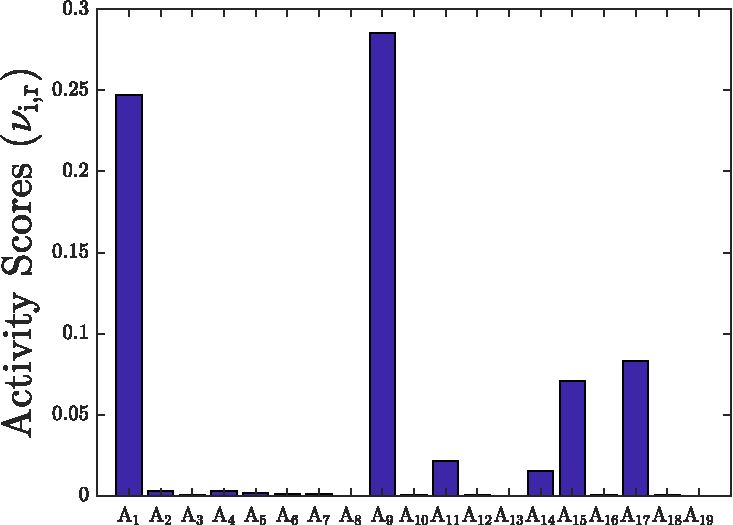
\includegraphics[width=0.45\textwidth]{./Figures/as_A_33D}
    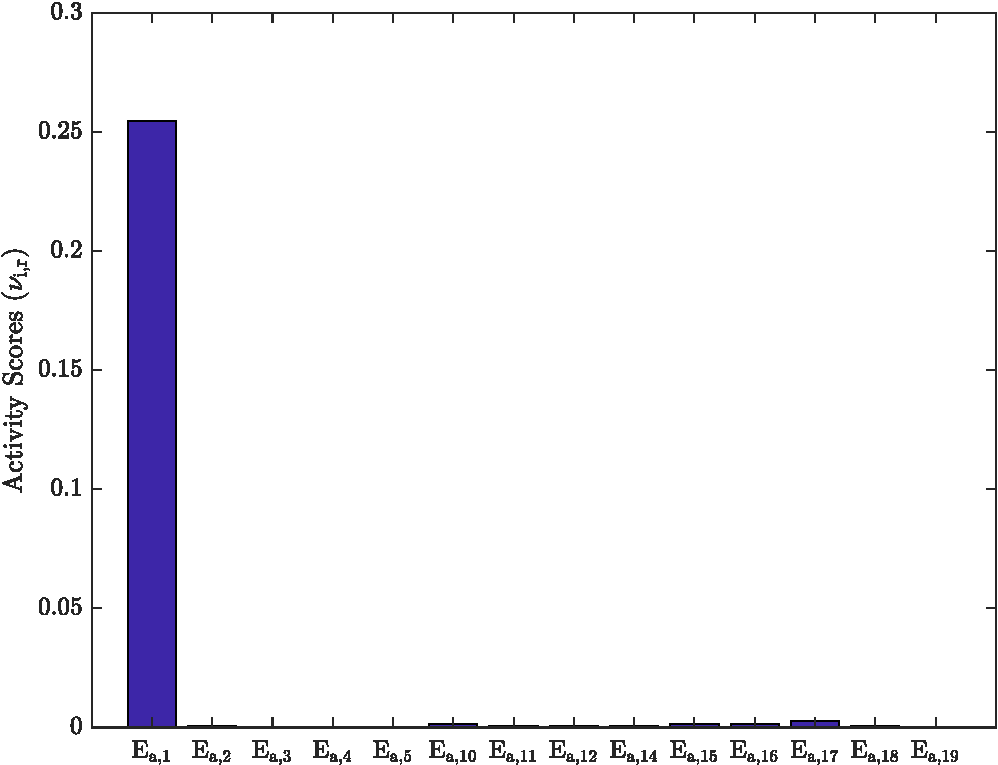
\includegraphics[width=0.45\textwidth]{./Figures/as_E_33D}
\caption{A bar-graph illustrating individual activity scores for the uncertain $A_i$' (left) and $E_{a,i}$'s (right).}
\label{fig:as_33D}
\end{center}
\end{figure}
%
From the above plot, it can be inferred that the ignition delay is predominantly sensitivity towards $A_1$, $A_9$, and
$E_{a,1}$. Furthermore, it is moderately sensitivity towards $A_{15}$ and $A_{17}$ while sensitivity towards remaining
inputs is found to be low or negligible. Note that the sensitivity results for the pre-exponents is found to be consistent
with the 19-dimensional case presented in~\ref{sec:method}. This observation can also be exploited for reducing the 
dimensionality of the problem from 33 to 3-5 depending upon the required level of accuracy in terms of characterizing 
the uncertainty in the model output. The sensitivity-driven dimension reduction for uncertainty quantification has been
discussed in our earlier effort~\cite{Vohra:2018}. In this work, however, we focus on dimension reduction using the active 
subspace approach which is shown to yield even greater scope for dimension reduction i.e. from 33 to 1. We verify
the accuracy of the 1-d regression fit to $G(\hat{\mat{W}}_1^\top\bm{\xi})$ in the following section.

\subsection{Surrogate Verification}
\label{sub:verify}

The 1-dimensional surrogate ($\mathcal{Y}$) is investigated for its accuracy as well as the ability to capture the 
uncertainty in the
model output in two ways. Firstly, we estimate the relative L-2 norm of the discrepancy~($\varepsilon_d$)
between estimates of ignition delay in the case of H$_2$/O$_2$ reaction, obtained using the 
model output and the surrogate in the following equation:
%
\be
\varepsilon_d = \frac{\|f(\bm{\theta}) - \mathcal{Y}(\bm{\xi})\|_2}{\|f(\bm{\theta})\|_2}
\ee
%
The relative norm, $\varepsilon_d$ was estimated to be 8.92$\times10^{-2}$ based on a validation test data
comprising 1000 model evaluations. Hence, in the norm-sense, it can be said that the 1-dimensional surrogate is 
reasonably accurate. 

Secondly, we verify the accuracy of the surrogate in a probabilistic setting. In particular, we compare a histogram
plot of the model evaluations for ignition delay in the validation set with a PDF of the same using the 1-dimensional
surrogate as shown in Figure~\ref{fig:pdf_33D}.
%
\begin{figure}[htbp]
 \begin{center}
  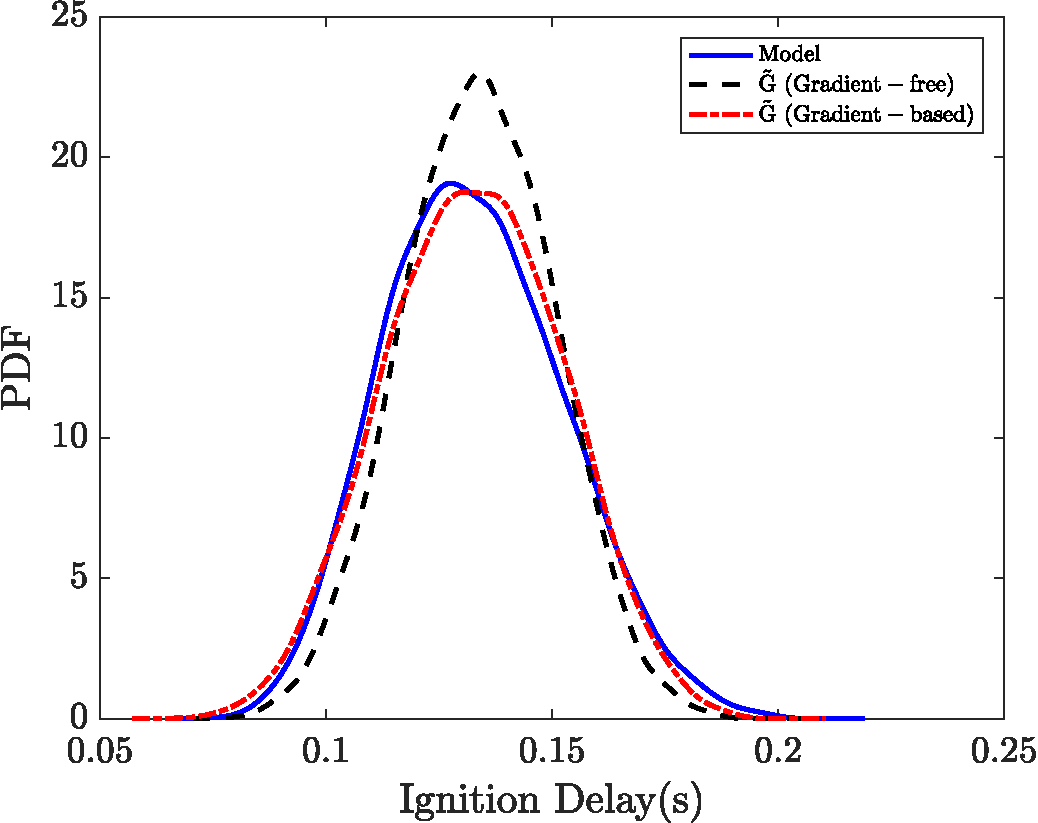
\includegraphics[width=0.45\textwidth]{./Figures/pdf_comp_id_1e4}
\caption{A comparison of the histogram plot based on model evaluations and the PDF based on surrogate
predictions for ignition delay. The two plots are based on samples in the validation set.}
\label{fig:pdf_33D}
\end{center}
\end{figure}
%
In the above comparison, it is observed that the peak of the PDF generated using the 1-dimensional surrogate in the
active subspace is consistent with the modal estimate based on the histogram. Moreover, the spread in the ignition
 delay is reasonably captured by the PDF. Hence, the surrogate is also verified in a probabilistic sense. 
 






























